\documentclass[border=4pt]{standalone}
\usepackage{amsmath,amssymb}
\usepackage{tikz}
\usetikzlibrary{arrows.meta}
\begin{document}
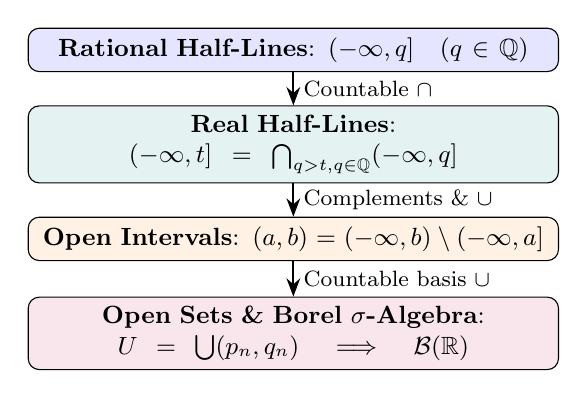
\begin{tikzpicture}[font=\small, >=Stealth]
  \node[draw, rounded corners, fill=blue!10, text width=6.5cm, align=center] (S1) at (0, 3.6)
    {\textbf{Rational Half-Lines}: $(-\infty, q] \quad (q \in \mathbb{Q})$};
  \node[draw, rounded corners, fill=teal!10, text width=6.5cm, align=center] (S2) at (0, 2.4)
    {\textbf{Real Half-Lines}: $(-\infty, t] = \bigcap_{q > t, q \in \mathbb{Q}} (-\infty, q]$};
  \node[draw, rounded corners, fill=orange!10, text width=6.5cm, align=center] (S3) at (0, 1.2)
    {\textbf{Open Intervals}: $(a,b) = (-\infty, b) \setminus (-\infty, a]$};
  \node[draw, rounded corners, fill=purple!10, text width=6.5cm, align=center] (S4) at (0, 0.0)
    {\textbf{Open Sets \& Borel $\sigma$-Algebra}: $U = \bigcup (p_n, q_n) \implies \mathcal{B}(\mathbb{R})$};

  \draw[->, thick] (S1) -- node[right, font=\footnotesize] {Countable $\cap$} (S2);
  \draw[->, thick] (S2) -- node[right, font=\footnotesize] {Complements \& $\cup$} (S3);
  \draw[->, thick] (S3) -- node[right, font=\footnotesize] {Countable basis $\cup$} (S4);
\end{tikzpicture}
\end{document}